%TC:envir minttcb [ignore] xall

\chapter{Custom Aircraft}\label{chp:custom_aircraft}

% Of the two, customizing aircraft is far more involved, and thus is the focus throughout the chapter.
It is quite possible that the vehicles, vehicle functionalities, or the environments that are provided by VTOL-AirSim are not sufficient for the needs of your project. In this case, there exists the option of customizing VTOL-AirSim beyond what it currently offers. This chapter and the next will teach you how to customize VTOL-AirSim. This chapter demonstrates how to create custom eVTOL aircraft, and the next chapter, Chapter~\ref{chp:custom_envs}, is dedicated to creating custom environments.

Because this topic can be quite broad, we have chosen to structure these two chapters on customization around guiding you through specific examples. Following our examples will allow you to see the entire process from start to finish. We begin with a discussion on a few general principles about meshes, after which we focus for the rest of the chapter on a specific example of taking a new eVTOL aircraft mesh all the way to flying it in VTOL-AirSim.

For dealing with meshes on Linux, we recommend the free 3D modeling software tool \textit{Blender}. See Appendix~\ref{apdx:blender} for more information about Blender and how to get it. You will need to install Blender in order to make some small adjustments to the example mesh before it can be properly used in Unreal Engine.

\section{Meshes}\label{sec:meshes}
As explained in Section~\ref{sec:definitions}, a \textit{mesh} is the collection of vertices, edges, and faces that make up the graphical representation of an object. Only one mesh is provided for each type of vehicle in VTOL-AirSim. For the \verb|Vtol| vehicle, we added a simple mesh of a tiltrotor aircraft (Fig.~\ref{fig:tiltrotor_mesh}). The UE4 assets for the aircraft are contained in the VTOL-AirSim repository.

\begin{figure}[t]
    \centering
    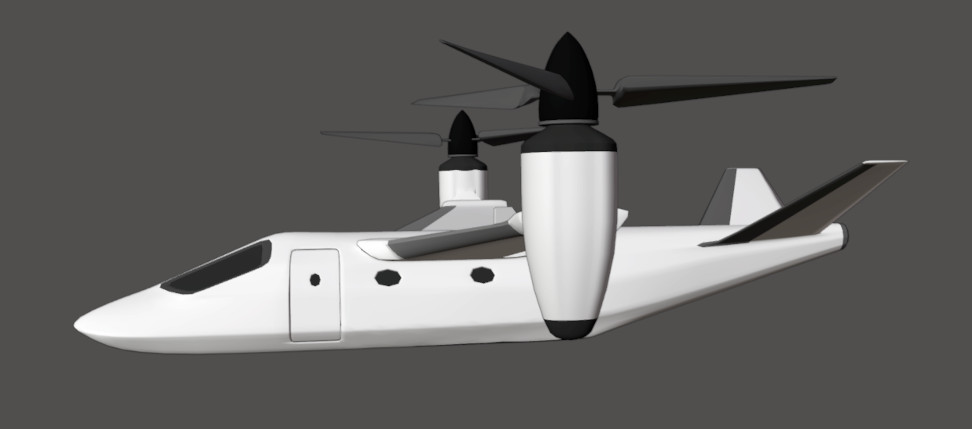
\includegraphics[width=\textwidth]{figures/tiltrotor_mesh}
    \caption[Default tiltrotor mesh]{
        The tiltrotor mesh that is provided for the \ci{Vtol} simulation mode in VTOL-AirSim.}%
    \label{fig:tiltrotor_mesh}
\end{figure}

Before we teach how to create a custom mesh, we wish to reiterate that the mesh of a vehicle is separate from the aircraft's actual dynamic model. It is simply a visual representation of the aircraft, which may or may not be an accurate representation of the vehicle's dynamics, current kinematic state, control outputs, etc. It is up to the developer to decide how the underlying model should affect the mesh, and to do the necessary work for accomplishing that. Customizing the mesh of a vehicle is a rather complicated and laborious task, even for simple cases. Therefore, you should first consider whether the needs of your project do indeed require a custom aircraft mesh or whether changing the model of the aircraft --- i.e., parameters such as mass, aerodynamic coefficients, the placement of motors, etc. --- would be sufficient. If you only need to change the model, see the VTOL-AirSim GitHub repo for instructions on how to do that.

\subsection{Obtain a Mesh from the Internet}
Modifying the geometry of a mesh is not a straightforward process. We therefore recommend seeking online for a mesh that fits your project well and requires the least amount of modifications as possible. There is a large and ever-growing number of 3D meshes available on the internet which have been created and shared by other people. In the vast majority of cases, obtaining an off-the-shelf mesh that works for your use case will save you a considerable amount of time and effort.

One place to look for downloadable meshes is the official Unreal Engine Marketplace. With this option, you will receive Unreal asset files can be placed directly into an Unreal Project. However, because downloading a mesh from the Unreal Marketplace into an Unreal Project requires using the Epic Games Launcher --- an app only available for Windows or MacOS --- we recommend looking at third-party 3D model sharing websites first (see Chapter~\ref{chp:custom_envs} for instructions on obtaining assets from the UE Marketplace). A few examples of websites for sharing 3D meshes include \url{turbosquid.com}, \url{cgtrader.com}, and \url{sketchfab.com}. These and other similar websites contain large databases of meshes made by other people that you can download. You can explore their selections by entering search terms on their website or by viewing categories such as \textit{Aircraft} or \textit{Vehicles}.

Many of the meshes hosted on these websites are not free; nevertheless, the cost is modest compared to the time required to create one from scratch, so do not let the price steer you away from a mesh if it fits well with the requirements of your project.

As you search for an appropriate mesh, there are two things you will want to look out for: the number of polygons (also called \textit{triangles}) and the file types offered. A very high number of polygons in the mesh could cause performance issues, which might manifest itself as slowing down interactions with the Unreal Editor, or possibly slowing performance in the simulation itself. What constitutes a ``very high number'' is entirely dependent on the computer hardware in question, whether it be your machine, or the machines of others; for instance, consider those who will be working with the mesh, or those who might run simulations containing the mesh. A good rule of thumb could be to look for meshes that have less than 200,000 polygons; though that is by no means a strict limit. For a point of reference, we have tested a mesh that consisted of 440,000 polygons in a VTOL-AirSim simulation that was handled well by some machines, but on other machines it resulted in performance lags and long loading times.

Lastly, try to find a mesh that is offered in \ci{.blend} format for use with the 3D modeling software Blender. This is because nearly all meshes will require some adjustments before they can be properly used in Unreal Engine. If the mesh you find is not offered as Blender project files, you can also download the mesh in a file format that can be imported into Blender, but the import process is not guaranteed to produce a clean result.

For a mesh to be imported into UE4, it must be in FBX format. Thus, there is a possibility that you could be successful in importing a mesh directly into UE4 as an FBX file. However, in our experience, this has resulted in problems such as meshes oriented in the wrong direction, or that the axis of rotation is oriented or positioned incorrectly when animating parts of the mesh --- for example, when animating the tilt of the rotors. We therefore recommend that you open the mesh in Blender first, then export the mesh to an FBX file.

\subsection{Creating a Mesh With CAD Software}
It is also possible to create a mesh from the ground up using CAD software. If you do choose to go this route, you will still need to import the mesh into Blender in order to export it in FBX format. One way to accomplish this is to export the mesh from the CAD program as a \ci{.wrl} file (also known as VRML, or Virtual Reality Modeling Language file format), then import the resulting \ci{.wrl} file into Blender, then export from Blender to FBX format. For an example of a mesh that was created in SolidWorks and was successfully brought into UE4 using this process, see the Maker aircraft files on the MAGICC Lab's Box storage at \url{https://byu.box.com/v/magicc-maker}.

\section{Edit a Mesh in Blender}\label{sec:blender_example}

We will now walk through an example of how to take a mesh obtained from the internet and get it to fly in VTOL-AirSim. For this example, we downloaded a free mesh of a tiltrotor aircraft from \url{turbosquid.com} and placed it in the MAGICC Lab Box storage. It is available for download at \url{https://byu.box.com/v/magicc-airsim-example-mesh}. Download this ZIP file and extract it to somewhere on your machine. Note that beyond this point you will need to have Blender installed.

After extracting the ZIP file, navigate to inside of the \ci{convertiplane} folder. The contents that you see are exactly as they appeared when the mesh was first downloaded, and the files are unmodified from the originals. The actual mesh is contained in the \ci{convertiplane.blend} file. Create a copy of this file and name it \ci{aircraft.blend}. Assuming that you have already installed Blender on your machine, start Blender and open \ci{aircraft.blend}.

At the top of the window, you will notice a number of tabs with names such as \textbf{3D View Full}, \textbf{Animation}, \textbf{Compositing}, \textbf{Default}, and others. These are called \textit{workspaces}. Let's create a new workspace of type \textit{Layout}. Click the plus icon to create a new workspace and select \textbf{General > Layout}.

\subsection{Delete Unnecessary Objects}
Let's delete objects from this mesh that are not needed. In the top-right is the \textbf{Outliner} panel that lists all the objects in the scene and their hierarchies. Find the \ci{convertoplan} (\textit{sic}) object and click the arrow to the left of its name to expand it. Next, expand the \ci{b3} object that is nested inside of \ci{convertoplan}. Hold the Shift key and select \ci{b3} and everything inside \ci{b3}, then press Delete. Repeat this for all of the objects in \ci{Collection 5}, \ci{Collection 14}, and \ci{Collection 15}. After removing these objects, you should have a screen similar to Fig.~\ref{fig:blender_begin}.

\begin{figure}[t]
    \centering
    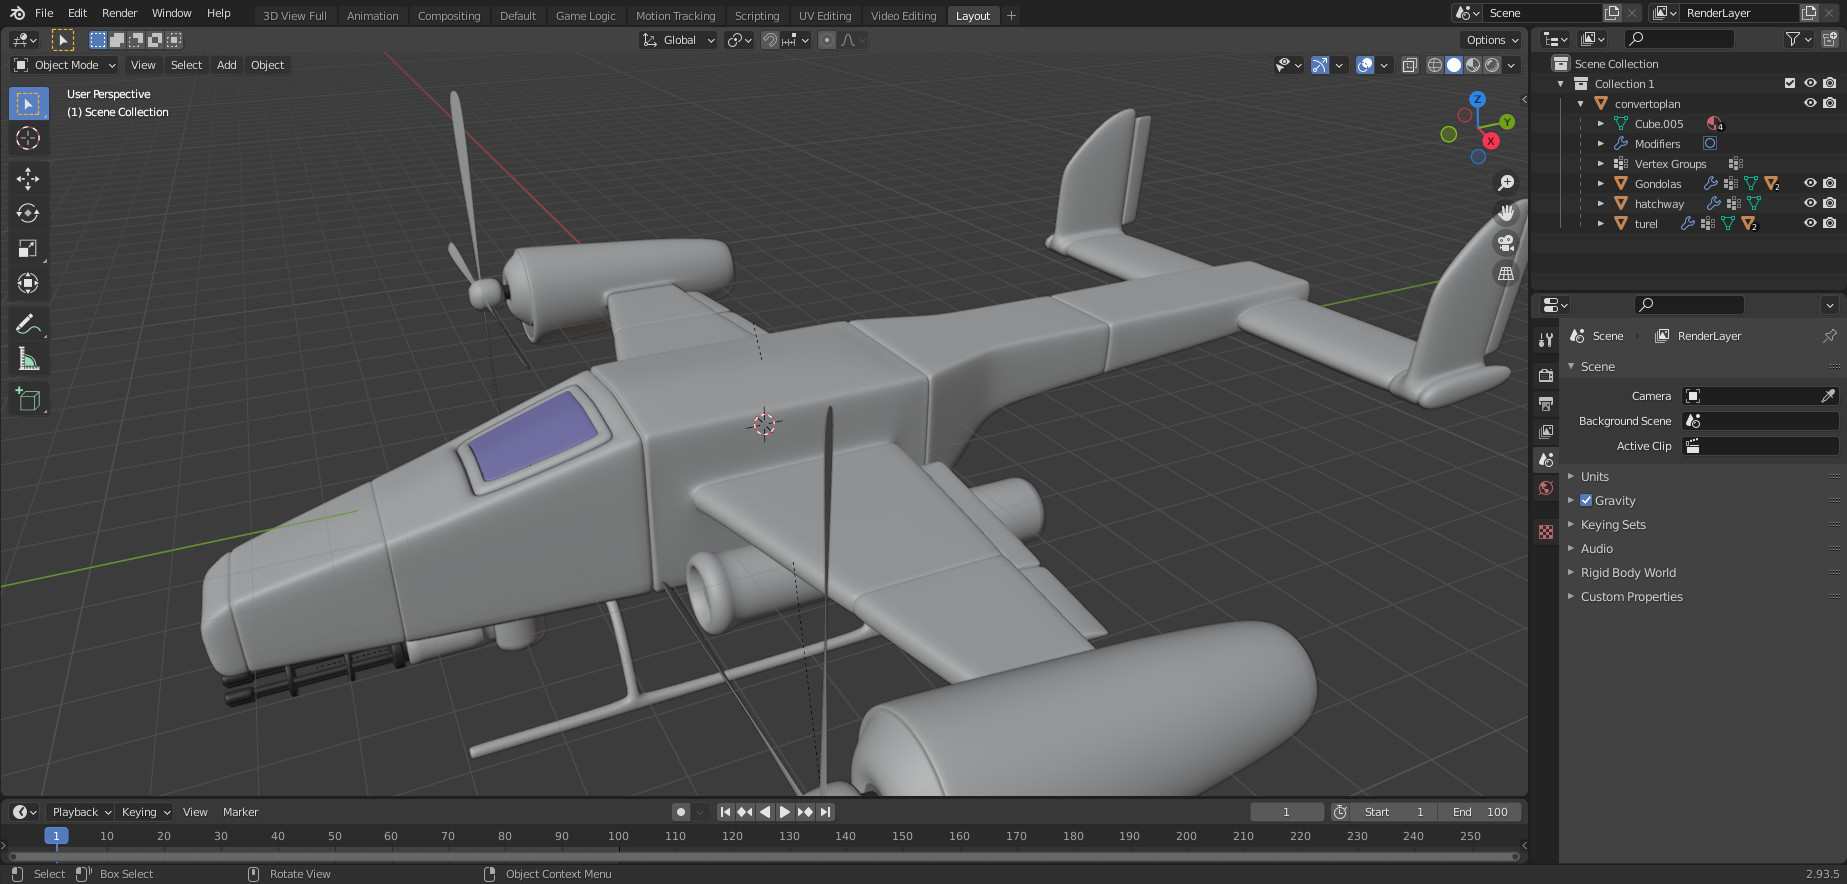
\includegraphics[width=\textwidth]{figures/blender_begin_alt}
    \caption[Blender screen of example VTOL mesh]{
        The example VTOL mesh open in Blender after removing unneeded objects.}%
    \label{fig:blender_begin}
\end{figure}

\subsection{Set the Zero Configuration}
We want forward for the aircraft to point in the +X (positive X) direction for importing into UE4. Click on the \ci{convertoplan} object to select it. Find the bottom-right \textbf{Properties} panel located directly underneath the \textbf{Outliner} and click the orange square icon to open \textbf{Object Properties}. Change each of the X, Y, and Z Location values to 0, and change the Rotation Z value to 90. Next, move your mouse over to the \textbf{Viewport} area, which is the panel currently displaying the mesh. Press the \texttt{A} key to select all objects. Press the key combination \texttt{Ctrl+A}, then click \textbf{Rotation} from the pop-up menu to apply the new rotation.

Now click on the \ci{Gondolas} object. We will refer to these cylindrical meshes as the \textit{engines}. In UE4, we will animate tilting the propellers by tilting the engines, which the propellers will follow. We want the zero rotation of the engines to be vertical, as this is what VTOL-AirSim expects. With \ci{Gondolas} selected, change the Rotation Y value to -90 and press \texttt{Enter}. Again, apply the rotation: mouse over to the \textbf{Viewport} area, press \texttt{Ctrl+A}, then click \textbf{Rotation} from the pop-up menu.

\subsection{Edit the Engines}
Select the \ci{Gondolas} object again. Notice that the two engines are a single object in Blender; we will need independent control of the tilt of each engine, so let's split the engines into two objects. In the upper-left of the \textbf{Viewport}, click \textbf{Object Mode} and select \textbf{Edit Mode}. You should now be able to see all the vertices, represented as black points, that make up the mesh of the engines. For the next part, let's move to a back view of the aircraft: in the upper-right of the \textbf{Viewport}, look for a graphic showing the global axes in red, green, and blue, and click on the hollow red circle (labeled \textbf{-X} when the holding the pointer over it). Also in the upper-right of the \textbf{Viewport} is an icon with two squares named \textbf{Toggle X-Ray}; click this icon to allow seeing all the vertices simultaneously. We can choose to separate either of the engines, so let's arbitrarily choose to separate the right engine. Draw a box around all the vertices of the right engine. You should now have a screen similar to Fig.~\ref{fig:blender_vertices} where all the vertices of the right engine are highlighted orange. Make sure your mouse is over the \textbf{Viewport} area, press \texttt{P}, then click \textbf{Selection} from the pop-up to create a new object. Change from \textbf{Edit Mode} back to \textbf{Object Mode} and click \textbf{Toggle X-Ray} to turn it off.

\begin{figure}[t]
    \centering
    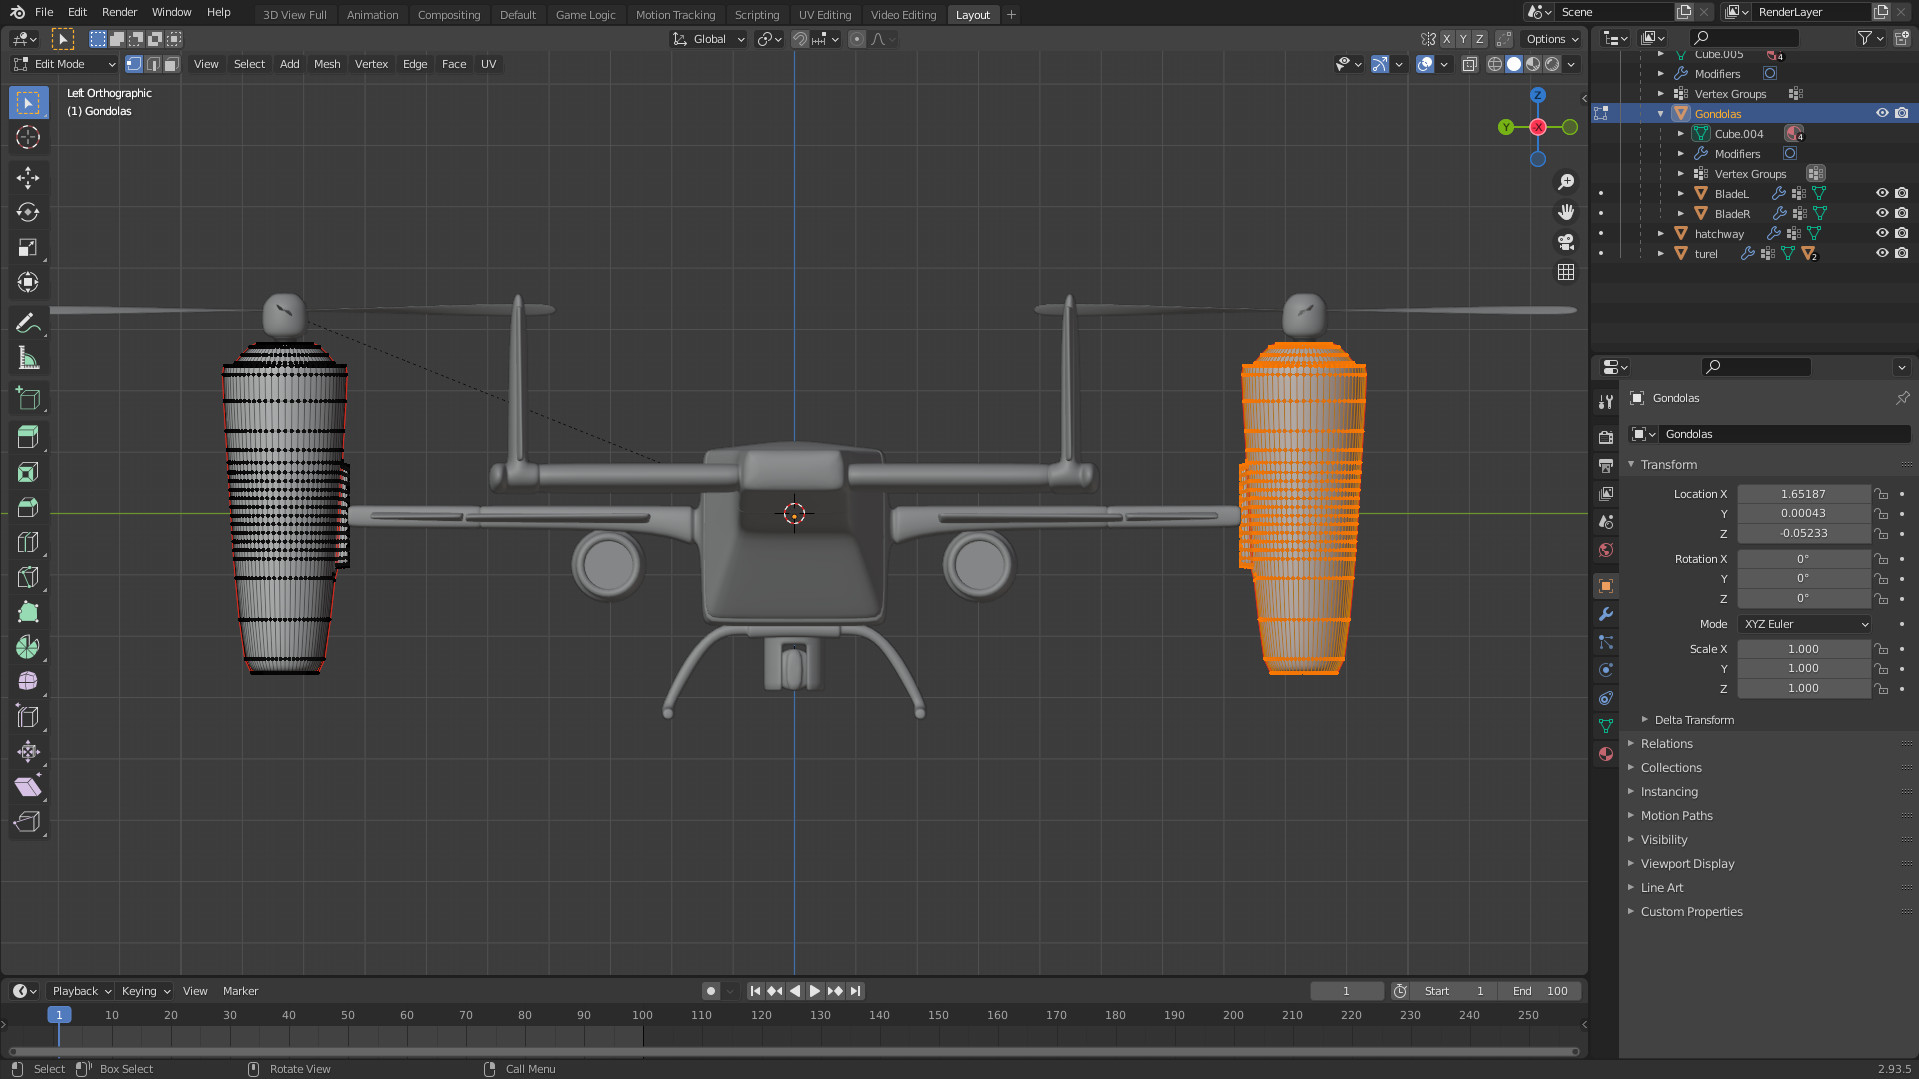
\includegraphics[width=\textwidth]{figures/blender_highlight_vertices}
    \caption[Blender screen of highlighted vertices]{
        This is how the screen should look in Blender after selecting the right engine's vertices.}%
    \label{fig:blender_vertices}
\end{figure}

In the \textbf{Outliner}, you should see an object named \ci{Gondolas} and a new object named \ci{Gondolas.001}. Rename \ci{Gondolas} to \ci{GondolaL} and \ci{Gondolas.001} to \ci{GondolaR}. Expand both \ci{GondolaL/R} objects, and find the \ci{BladeL/R} objects under \ci{GondolaL}. Click and drag \ci{BladeR}, then, while dragging, begin pressing \texttt{Shift+Alt}, and finally drop it onto \ci{GondolaR}. Doing this \textit{reparents} \ci{BladeR} to \ci{GondolaR}. Next, click and drag \ci{GondolaL}, then again press \texttt{Shift+Alt} while dragging, but this time drop it onto \ci{Collection 1}. Repeat this process for \ci{GondolaR}. This will clear their parent, which is needed to avoid a problem that occurs with nested hierarchies when exporting to FBX format.

\subsection{Move Origins of the Propellers}\label{sec:origins_props}
Next, we will fix the origins of the propellers. These origins will become the pivot points in UE4. Hold the \texttt{Ctrl} key and, in the \textbf{Outliner}, select \ci{BladeL} and \ci{BladeR}. In the top-left of the \textbf{Viewport}, click \textbf{Object} to reveal the \textbf{Object Menu}. Select \textbf{Set Origin > Origin to Geometry}. Let's also reset the zero rotations for all objects as their current rotations: hold your pointer over the \textbf{Viewport}, press \texttt{A} to select all objects, press \texttt{Ctrl+A} then click \textbf{Rotation}.

\subsection{Fix Object Names}
Finally, let's fix some object names. Rename \ci{convertoplan} to \ci{body}. With \ci{body} expanded, you will see an \textit{Object Data} item with a green triangle mesh icon named \ci{Cube.005}. Give it the same name of \ci{body}. Now do the same for the Object Data items under \ci{GondolaL}, \ci{GondolaR}, \ci{BladeL}, and \ci{BladeR} by renaming them to \ci{GondolaL}, \ci{GondolaR}, etc., respectively. Make sure each object is expanded in order to see its Object Data item. After finishing, press \texttt{Ctrl+S} to save the file.

\subsection{Export to FBX}
The mesh is ready for export. Go to \textbf{File > Export > FBX (.fbx)} to open the exporting utility window. On the right column of the window is a list of options. Under \textbf{Include} and \textbf{Object Types}, hold \texttt{Shift} and click \textbf{Mesh} and \textbf{Other}. Under \textbf{Transform} and \textbf{Up}, change the value to \textbf{Z Up}. Uncheck the option \textbf{Use Space Transform}, and check the box for \textbf{Apply Transform}. Next, expand the \textbf{Geometry} section and set \textbf{Smoothing} to \textbf{Face}. After that, you should have the settings shown in Fig.~\ref{fig:blender_fbx_export}. Finally, keep the file name as \ci{aircraft.fbx} and click \textbf{Export FBX}.

\begin{figure}[t]
    \centering
    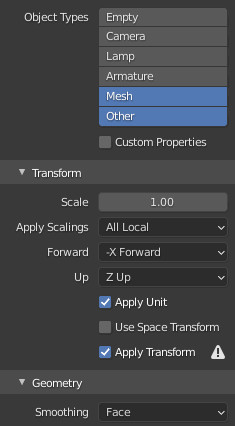
\includegraphics[height=230pt]{figures/blender_fbx_export}
    \caption[The required FBX export settings in Blender]{
        These are the required settings when exporting to FBX from Blender.}%
    \label{fig:blender_fbx_export}
\end{figure}

\section{Import Mesh Into UE4}\label{sec:import_mesh_ue4}
Once you have an FBX file of the mesh, it is time to import it into a project using Unreal Editor. In this section, we will import the mesh that we exported from Blender in the previous section. To make the instructions easier to follow, let's give a simple, memorable name to the aircraft: Homer, after the ancient Greek poet.

We will begin by creating a new Unreal Project that we can modify for this extended example by making a copy of the Blocks project. Navigate to where you have the Blocks project on your file system and create a simple copy named \ci{Blocks_test}. We want UE4 to rebuild the project, so we need to delete the \ci{Binaries}, \ci{Intermediate}, and \ci{Saved} folders in both the \ci{Blocks_test} and the \ci{Blocks_test/Plugins/vtol-AirSim} folders. The \ci{vtol-AirSim} folder also has a script named \ci{clean.sh} that you can use to automate the removal.

Start Unreal Editor and open the newly created project. To open it, do the following: if Unreal Editor is showing you the \textbf{Unreal Project Browser} window, click \textbf{More} and then \textbf{Browse}; else, if you already have a project opened, go to \textbf{File > Open Project} and then click \textbf{Browse}. Navigate to the \ci{Blocks_test} project and double-click on the file \ci{Blocks.uproject}. In the dialog that appears asking if you would like to rebuild the missing modules of Blocks and AirSim, click \textbf{Yes}.

Once the Blocks\_test project is opened, look at the \textbf{Content Browser} and ensure that \textbf{View Options > Show Plugin Content} is checked. In addition, show the \textbf{Sources panel} by clicking the icon to the left of the \textbf{Filters} icon. Now look at the \textbf{Sources panel} and navigate to \ci{AirSim Content/VTOL}. Create a folder here for the new aircraft by pressing \texttt{Ctrl+Shift+N}. Name the folder \ci{Homer}. Move inside the \ci{Homer} folder and create two new folders named \ci{Meshes} and \ci{Blueprints}.

Next, let's import the mesh. Go to \textbf{File > Import Into Level}. In the file browser dialog, find the \ci{aircraft.fbx} file that you exported from Blender earlier. In the next dialog, choose the import location as \ci{AirSim Content/VTOL/Homer/Meshes}. The next dialog will show a number of options. Under \textbf{Import Options}, check the boxes for \textbf{Import as Dynamic} and \textbf{Force Front XAxis}, then click \textbf{Import}.

A new editor window will open titled \textbf{FbxScene\_aircraft}. We will discuss this window in the the next section, so for now, return to the main Unreal Editor window. You should see the \ci{Meshes} folder populated with a number of assets. Note that these new assets are of four types: \textit{Material}, \textit{Static Mesh}, \textit{Blueprint Class}, and \textit{Fbx Scene Import Data}. The type of each asset is indicated by a colored accent along the bottom of the asset's thumbnail: green for Material, cyan for Static Mesh, blue for Blueprint Class, and purple for Fbx Scene Import Data. You can also hover your mouse pointer over any asset and the pop-up that appears will display the asset's name followed by its asset type in parentheses; for example, if you hover over the \ci{body_001} asset, it will display the title \textit{body\_001 (Static Mesh)}.

The various materials and the component meshes for the tiltrotor aircraft were originally defined in Blender, and Blender exported data about the parts and materials of the mesh into FBX format.  When Unreal Editor imported the FBX file, it tried to interpret the data and create assets that represent what is contained in the data. This process isn't perfect, and you may find that there are discrepancies between what is you can see in the scene in Blender compared with what is generated in UE4 by importing the FBX file. In this example, we won't import any textures; however, in general, you can also import the texture files supplied for a mesh (in the form of image files) separately and apply them in UE4. An easy way to change the look of the aircraft is by making simple modifications to the materials, such as color, roughness, or how metallic they look. UE4 comes with its own Material Editor, so this method allows for changing the look of the aircraft mesh inside Unreal Editor rather than requiring external tools for editing.

\section{Make a Custom Blueprint}\label{sec:blueprint}
In Unreal Engine, \textit{Blueprints} is a visual scripting system that is used to accomplish a broad range of tasks. It is a way to do visual programming in that virtually anything that the UE4 \CC libraries can do can be done using Blueprints, and vice versa. Nevertheless, some things are more easily done in Blueprints, while others are more easily done in \CC code. If you are familiar with the \textit{LabView} visual programming system from National Instruments, they share some similarities. For our purposes of creating a controllable aircraft, you can also think of it as having similarities with what are called \textit{assemblies} in some CAD software. In addition, a Blueprint is interchangeably called a \textit{Blueprint Class} because it is a class in the same sense of the word's meaning in \CCd. You create an \textit{instance} of a Blueprint Class by spawning or placing an Actor in the level of that Blueprint Class. As an example, there is one \ci{TiltrotorPawn} \CC class and one \ci{BP_TiltrotorPawn} Blueprint for the tiltrotor vehicle, but we can spawn one or more tiltrotor vehicles in a simulation where each one has a different name, a different state, etc.

While almost everything in VTOL-AirSim is contained in the \CC code, a few aspects concerning the mesh animation is contained in the form of Blueprints. In particular, this includes:
\begin{itemize}
    \item The Static Meshes that are used to visually represent the aircraft
    \item The relationships between the meshes (i.e., the hierarchies and relative transforms)
    \item The mechanism which sets the rotation speed of the propellers
    \item The Materials assigned to each Material Slot
\end{itemize}

\subsection{Notes on Naming Conventions}
First, we wish to cover a few definitions and naming conventions. A \textit{Pawn} in Unreal Engine is defined as ``the base class of all Actors than can be controlled by players or AI''. All of the aircraft in VTOL-AirSim are derived classes of the Pawn \CC class, and thus have the naming convention of appending \textit{Pawn} to the class name. Each vehicle mesh consists of a Blueprint that inherits from one of the vehicle Pawn \CC classes. A Blueprint for a vehicle mesh has the prefix \textit{BP\_}, and this is how AirSim's multirotor vehicle and VTOL-AirSim's tiltrotor got the names \ci{BP_FlyingPawn} and \ci{BP_TiltrotorPawn}, respectively.

\subsection{Relative Transforms in Blueprints}
Section~\ref{sec:import_mesh_ue4} had you use the \textbf{Import Into Level} feature, and this tries to automatically create a Blueprint based on the data contained in the FBX file. This is the \textbf{FbxScene\_aircraft} Blueprint. Go back to the editor window for the Blueprint, or double-click on the asset in the \textbf{Content Browser} if you no longer have the window. In the Blueprint editor, switch to the \textbf{Viewport} tab. On the left of the window, you will see the \textbf{Components} panel which contains a hierarchy of \textit{Components} which make up the Blueprint that reflects the same hierarchy of objects that we saw in Blender. Click on the \ci{GondolaR} Static Mesh Component, then look at the \textbf{Details} panel on the right side of the window. Notice that its Location X, Y, and Z values reflect their values set in Blender, except that the Y-axis is negated and they are all multiplied by 100 --- this is because UE4 uses a left-handed North-East-Up coordinate system, and its base unit of length is the centimeter (Blender is unitless by default, but UE4's process of interpreting the FBX specification causes the values to be multiplied by 100, which is desirable in this case). However, you will see that the same is not true for \ci{BladeR}; the values are a bit different than in Blender. This is because in Blender the Location values are relative to the global coordinate frame (assuming that the Location transform has not been applied), while in UE4, the Location values are relative to the coordinate frame of its \textit{parent}, which in this case is \ci{GondolaR}.

\subsection{Origins (Pivot Points) of Meshes}
Understanding where the origin of a mesh (or \textit{pivot point}, as it is called in Unreal Engine) comes from is very important, because \textit{there is no way to change the origin (pivot point) of a mesh in Unreal Engine}. The pivot point of each Static Mesh is read by UE4 at the time of import and then becomes fixed, both its position and orientation, after the asset is generated. This is why we set the origins of the propeller objects to be at their geometric centers in Section~\ref{sec:origins_props}, as it is only in Blender (or some other 3D modeling software) that the position of the point can be changed, as well as the orientation of the coordinate axes with respect to the mesh. If you are having problems getting the right pivot points for meshes, see Appendix~\ref{apdx:blender_origins_alt} for an alternate method of correcting origins in Blender.

\subsection{Create a New Blueprint}
Each unique vehicle must have its own Blueprint to fly in VTOL-AirSim. We could modify the \ci{FbxScene_aircraft} Blueprint that UE4 created for us, but this would require more work than modifying a copy of the \ci{BP_TiltrotorPawn} Blueprint, so we will do the latter.

Copying a Blueprint must be done in Unreal Editor. In the \textbf{Content Browser}, navigate to the folder \ci{AirSim Content/VTOL/Tiltrotor/Blueprints}. With the \textbf{Sources panel} open, click and drag the \ci{BP_TiltrotorPawn} asset to the \textbf{Sources panel} and drop it onto the \ci{VTOL/Homer/Blueprints} folder, then select \textbf{Copy here} from the pop-up. Navigate to that same folder and rename the copied Blueprint to \ci{BP_HomerPawn}, then double-click it to open the Blueprint Editor. Click on the \textbf{Viewport} tab in the Blueprint Editor so you can see the changes we will make in the next steps.

\subsection{Replace the Static Mesh Components}
At this point, you should see the default tiltrotor aircraft in VTOL-AirSim. Let's replace the Static Mesh Components in the Blueprint with the new aircraft mesh. Select all the Static Mesh Components under the \ci{Body} component by holding \texttt{Shift} while clicking on them, and press \texttt{Delete} to remove them. Next, click on the \ci{Body} component and find the \textbf{Static Mesh} property in the \textbf{Details} panel. To change it, click on the mesh name to reveal a drop-down list, begin typing \texttt{body}, and then select \ci{body_001} (or similarly named) from the filtered list. Now you should see the body of the new aircraft in the \textbf{Viewport}; the Static Mesh of the \ci{Body} Static Mesh Component (which is the Blueprint's Root Component) has now been set to the body of the new aircraft mesh.

\begin{figure}[t]
    \centering
    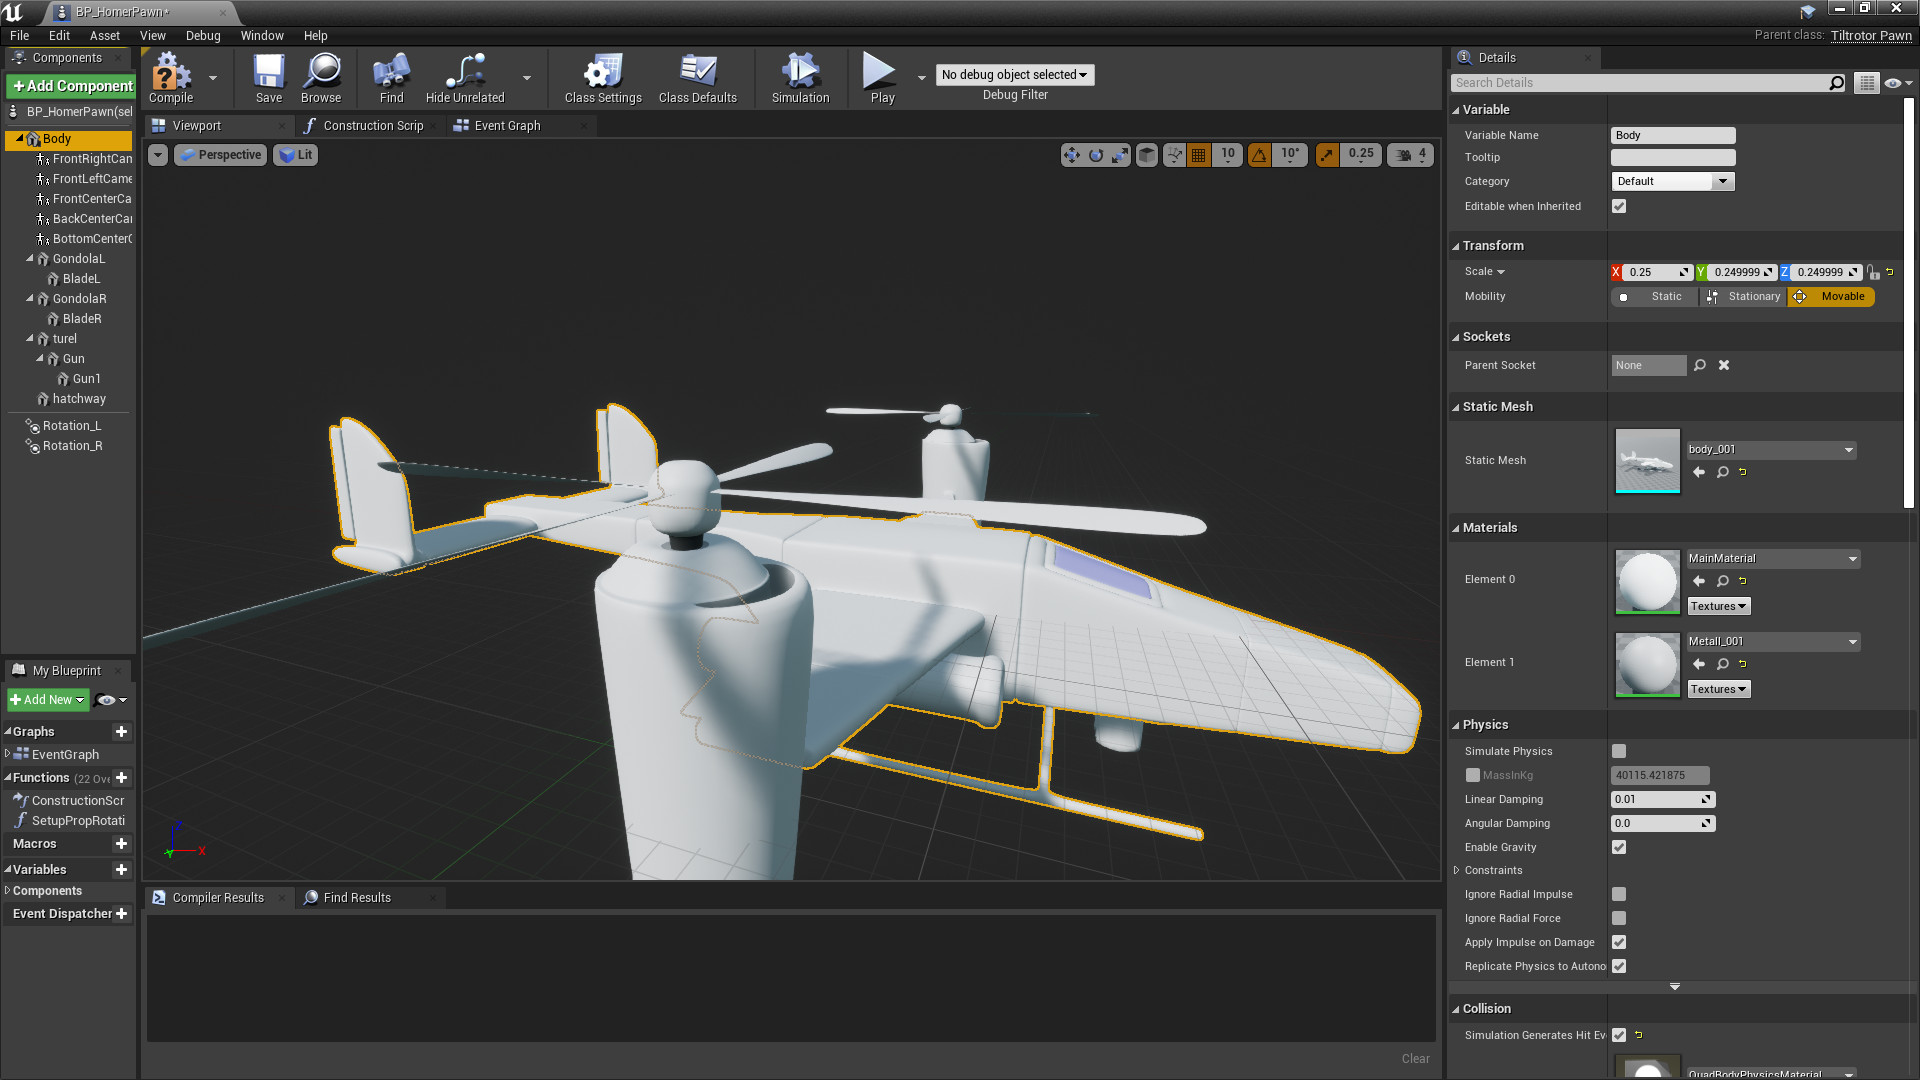
\includegraphics[width=\textwidth]{figures/ue4_blueprint_viewport}
    \caption[Viewport of Blueprint with example aircraft mesh]{
        The Viewport of \ci{BP_HomerPawn} after adding all of the new aircraft's Static Mesh Components to the Blueprint.}%
    \label{fig:ue4_blueprint_viewport}
\end{figure}

The next task is to copy the configuration of the Static Mesh Components contained in the \ci{FbxScene_aircraft} Blueprint to the \ci{BP_HomerPawn} Blueprint. Select all the Static Mesh Components in \ci{FbxScene_aircraft} using \texttt{Shift} and click, then right-click on any of the selected components and select \textbf{Copy}. In the editor for \ci{BP_HomerPawn}, right-click on \ci{Body} and select \textbf{Paste}. Finally, delete the \ci{body1} component from the components that you just pasted. You should now see the full aircraft mesh in the \ci{BP_HomerPawn} Viewport, as shown in Fig.~\ref{fig:ue4_blueprint_viewport}.

\subsection{Edit \texttt{SetupPropRotationMovement}}\label{sec:ue4_blueprint_setupprop}

There is one visual programming piece of the Blueprint that needs to be edited. In the \textbf{My Blueprint} panel located in the lower-left of the window, under the \textbf{Functions} section, find the function named \ci{SetupPropRotationMovement} and double-click it to open it in a new tab. Notice the two boxes titled \textbf{Set Updated Component} where the left and right boxes have connections to nodes labeled \textbf{Rotation L} and \textbf{Rotation R}, respectively. Hold your mouse pointer over the \textbf{Rotation L} node --- but not its label, rather over the empty space to the left of the label text --- and the tooltip tells you \textit{Read the value of variable Rotation\_L}. Indeed, this and the \textbf{Rotation R} node read the values from the \ci{Rotation_L} and \ci{Rotation_R} Rotating Movement Components of this Blueprint (see the \textbf{Components} panel) and feed those values as inputs to the \textbf{Set Updated Component} functions.

\begin{figure}[ht]
    \centering
    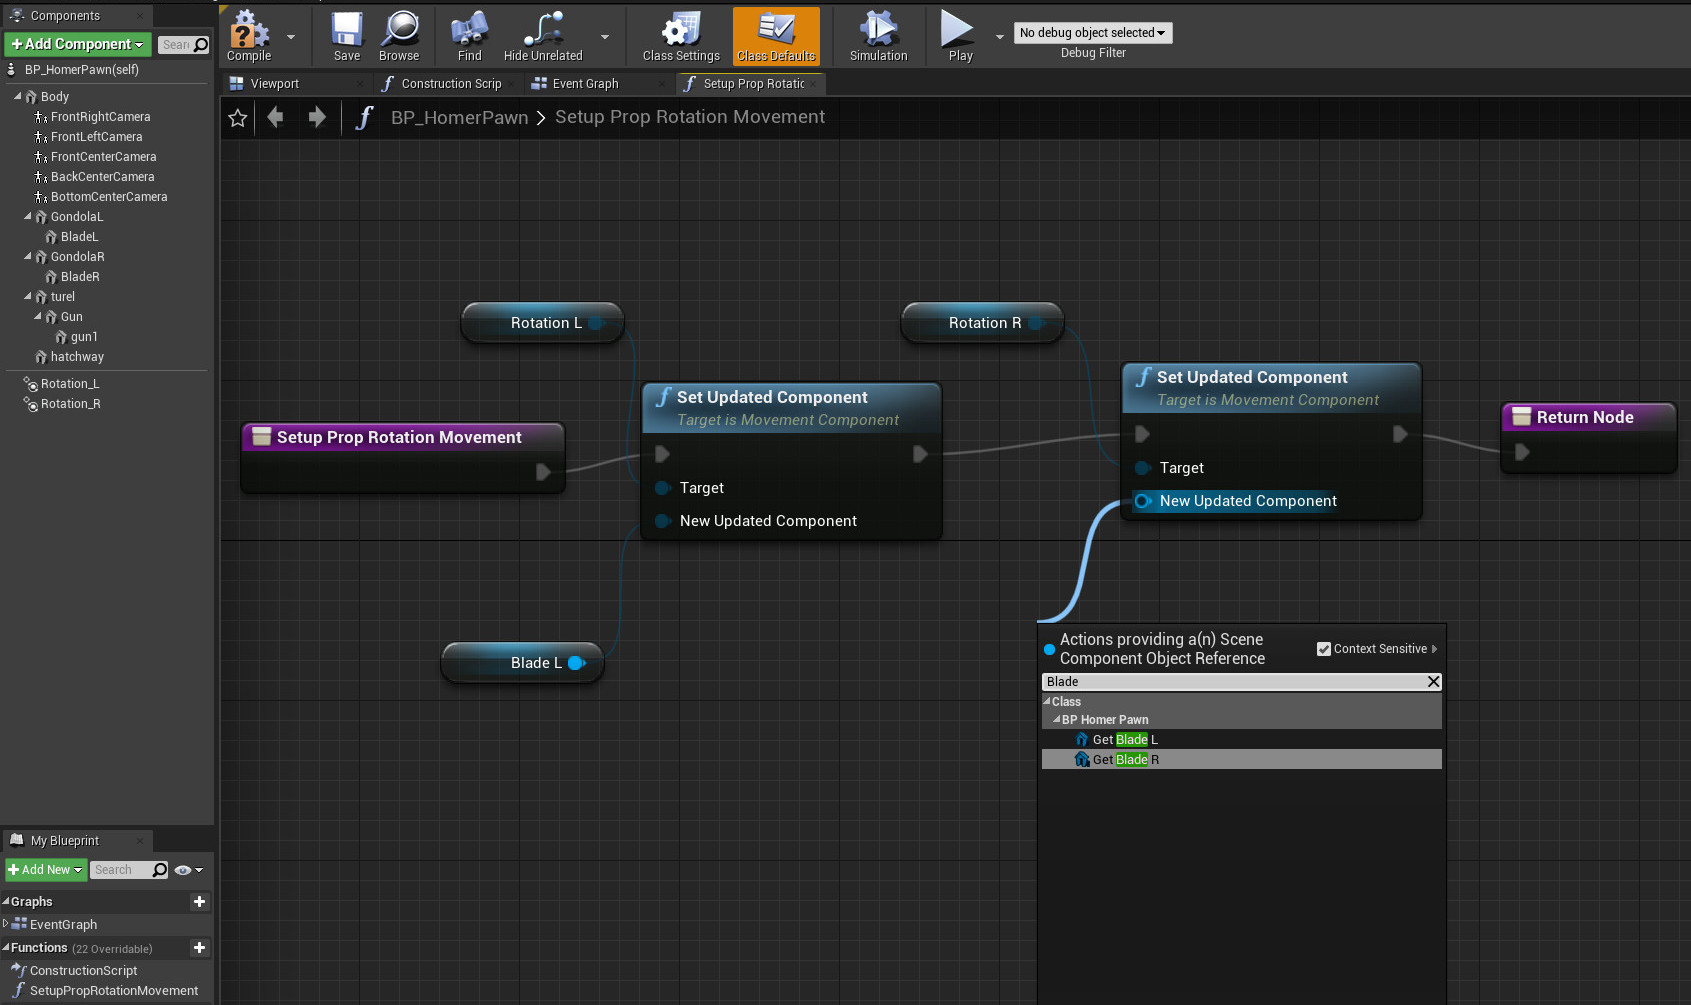
\includegraphics[width=\textwidth]{figures/ue4_blueprint_setupproprotation2}
    \caption[Editing the Blueprint function SetupPropRotationMovement]{
        In the \ci{SetupPropRotationMovement} function, what appears after clicking on the \textbf{New Updated Component} terminal, dragging outward, releasing, and then typing the search term \texttt{Blade}.}%
    \label{fig:ue4_blueprint_setupproprotation}
\end{figure}

If you look at the same function in \ci{BP_TiltrotorPawn}, you will see that the each box also has output connections going to nodes labeled \textbf{Prop L} and \textbf{Prop R}, which correspond to the \ci{Prop_L} and \ci{Prop_R} components of the Blueprint; these nodes and connections were present when we first copied the \ci{BP_TiltrotorPawn} Blueprint, but the nodes were deleted when we deleted the \ci{Prop_L/R} components.

What this function does is it links together the \textit{Rotating Movement Components} in the Blueprint to the Static Mesh Components that we want to animate. In UE4, a Rotating Movement Component is a non-scene component (i.e., it is not rendered and has no position) which simply ``performs continuous rotation of a component at a specific rotation rate''. AirSim uses Rotating Movement Components in order to set the speed that the propellers rotate. In the \CC code, it is the \ci{RotationRate.Yaw} of the Rotating Movement Components that get set by their calculated values based on control inputs in AirLib, and it is in this Blueprint function where each of the \ci{Rotation_L/R} components are linked to affect each of the propellers.

In \ci{BP_HomerPawn}, we simply need to have \ci{BladeL/R} be the outputs of the left and right boxes. To create output connections to new nodes for these boxes, click on the terminal (the hollow circle) of \textbf{New Updated Component} and drag downward toward any empty area and release; this will reveal a pop-up which allows you to search for the node you want to create (see Fig.~\ref{fig:ue4_blueprint_setupproprotation}). Type \texttt{Blade}, and click on \textbf{Get Blade L} for the left box, or \textbf{Get Blade R} for the right box. Follow this process for both boxes.

Once you have a connection from the \textbf{New Updated Component} terminal of the left box to \textbf{Blade L} and a connection from the right box to \textbf{Blade R}, you are finished with the Blueprint. Save your changes.

\section{Perform a Test Flight}
We are ready to perform the first test flight of the Homer aircraft in the Unreal Editor. First, you will need to place the following settings in your \ci{settings.json} file:
\begin{minttcb}[title={AirSim Settings For Custom HomerPawn Aircraft}]{json}
{
  "SettingsVersion": 1.2,
  "SimMode": "Vtol",
  "PawnPaths": {
    "DefaultVtol": {
      "PawnBP":
        "Class'/AirSim/VTOL/Homer/Blueprints/BP_HomerPawn.BP_HomerPawn_C'"
    }
  },
  "Vehicles": {
    "uav0": {
      "VehicleType": "VtolSimple"
    }
  }
}
\end{minttcb}
In the \ci{PawnPaths} setting, we specify what we want to use as the default Blueprint for all vehicles of type \ci{Vtol} (this can also be configured for each vehicle, if needed) so that AirSim will choose \ci{BP_HomerPawn} rather than the default \ci{BP_TiltrotorPawn}. The somewhat confusing string that is required to specify \ci{BP_HomerPawn} is due to how UE4 deals with paths within projects as well as how UE4 generates object names. In short, the class object for \ci{BP_HomerPawn} becomes \ci{BP_HomerPawn.BP_HomerPawn_C}, contained within the single quotes is the path string to the serialized object, and the text \ci{Class} means the object is of type \ci{Class} --- other types include \ci{Material}, \ci{StaticMesh}, etc. See Appendix~\ref{apdx:unreal_paths} for an explanation of path references in UE4.

After you have saved the \ci{settings.json} file, go back to Unreal Editor. In the \textbf{World Outliner}, find the \textbf{FbxScene\_aircraft} Actor that UE4 automatically placed in your level. Select it and press \texttt{Delete}. Next, click \textbf{Play} in Unreal Editor. You should see a \ci{BP_HomerPawn} Actor spawn in the Blocks world. In a terminal, run the geometric controller example from Section~\ref{sec:vtol_geometric_control}. After running the \ci{geometric_control_airsim_sim.py} script, you should see the aircraft take off and fly until it hits a wall. Notice that the propellers are spinning as they should, but the engines never tilt. Click \textbf{Stop} to end the simulation.

There is a very simple reason as to why the engines were not tilting: the names of the engines are hard-coded as \ci{Engine_L} and \ci{Engine_R} in the \CC code, yet HomerPawn's engines are named \ci{GondolaL/R}. There are two ways in which you can solve this problem: you can fix the names of the engine components in the Blueprint, or you can create a new \CC class for the Homer aircraft which uses appropriate names. In order to demonstrate how to create a new vehicle \CC class for those who may need more advanced customizations, we are going to do the latter option. If you do not think you will need to modify any of the VTOL-AirSim code for your project, then you can do the former option and stop there. Otherwise, close out of Unreal Editor and continue to the next section.

\section{Create a \texorpdfstring{\CCh}{C++} Class}\label{sec:cpp_class}
In this section, we create a replica of the \ci{TiltrotorPawn} source code and rename it to \ci{HomerPawn}. Then, we modify the code to correctly animate the tilting of the engines on the Homer aircraft mesh.

\subsection{Copy Files from TiltrotorPawn}
First, go to \ci{Blocks_test/Plugins/vtol-AirSim/Source/Vehicles}. Create a new folder and name it \ci{Homer}. From the \ci{Tiltrotor} folder, copy the files \ci{TiltrotorPawn.h} and \ci{TiltrotorPawn.cpp} into the \ci{Homer} folder and rename them to \ci{HomerPawn.h} and \ci{HomerPawn.cpp}.

Next, open VS Code in the folder \ci{Homer}. Press the keys \texttt{Ctrl+Shift+F} to search across all files in the opened directory. Type \texttt{Tiltrotor} into the \textbf{Search} box. Click the small arrow to the left of the search box to reveal the \textbf{Replace} box. Enter \texttt{Homer} as the replacement term. Click the \textbf{Replace All} icon to the right of the \textbf{Replace} box, or press the keys \texttt{Ctrl+Alt+Enter}. Click \textbf{Replace} in the dialog that appears.

There is one class that should keep its original name --- \ci{TiltrotorPawnEvents} --- as we don't need to change anything in it to be compatible with \ci{HomerPawn}. Repeat the same process to replace occurrences of \ci{HomerPawnEvents} with \ci{TiltrotorPawnEvents}. Lastly, in \ci{HomerPawn.h}, change the include statement from \ci{"TiltrotorPawnEvents.h"} to use the correct file path of \ci{"Vehicles/Tiltrotor/TiltrotorPawnEvents.h"}. With those changes, you now have a \CC class for \ci{HomerPawn} that can compile without errors.

\subsection{Correct Names of Engine Components}
We still need to fix the names of the engine components before the class will be fully functional. In VS Code, open \ci{HomerPawn.cpp} and find the two lines containing the strings \ci{"Engine_L"} and \ci{"Engine_R"}. Change each string to be \ci{"GondolaL"} and \ci{"GondolaR"}. Notice, in addition, the lines containing the strings \ci{"Rotation_L"} and \ci{"Rotation_R"}; this is where the Rotating Movement Components that we discussed in Section~\ref{sec:ue4_blueprint_setupprop} are specified. We don't need to change those strings because the component names remain the same in \ci{BP_HomerPawn}. Note also that these two arrays of components are looped over in the function \ci{SetRotorRenderedStates} later on in the file. This is where their values are set, and they are set according to the data contained in the vector \ci{rotor_infos}, which ultimately comes from AirLib.

This completes our changes to the code. Run the script \ci{clean.sh} in \ci{vtol-AirSim} and launch Unreal Editor. Open the \ci{Blocks_test2} project and click \textbf{Yes} on the dialog to rebuild the modules.

\subsection{Reparent the Blueprint}
Once Unreal Editor has rebuilt and opened the project, open \ci{BP_HomerPawn} again to make a necessary change. In the toolbar near the top of the Blueprint Editor, click on \textbf{Class Settings}. In the \textbf{Details} panel, find the \textbf{Parent Class} field and click on the field's current value of \textbf{Tiltrotor Pawn}. Begin typing \texttt{Homer} and you should see \textbf{Homer Pawn} appear from the list of filtered items. Select \textbf{Homer Pawn}, then click \textbf{Continue} on the dialog to reparent the Blueprint. The \textbf{Homer Pawn} class is the \ci{AHomerPawn} \CC class that you created; if it shows up in the list of classes, that means UE4 successfully built your new class. Lastly, save the changes to the Blueprint.

This step of reparenting creates the actual link between the \ci{BP_HomerPawn} Blueprint and the \ci{AHomerPawn} \CC class. Now, when a \ci{BP_HomerPawn} Actor is spawned, it will use your custom code in \ci{HomerPawn.cpp}.

\section{Improve the Look With Materials}
You are now ready for a fully functional test flight of the Homer aircraft. But before we do the final flight, let's improve the look of the aircraft by changing the Materials assigned to the Material Slots of the various components. We will do that by reusing Materials from the VTOL-AirSim tiltrotor aircraft.

In the Blueprint Editor for \ci{BP_HomerPawn}, make sure the \ci{Viewport} tab is active. In the \textbf{Components} panel, select the \ci{Body} component. Find the Material Slot named \textbf{Element 0} and click on the currently selected material named \textbf{MainMaterial}. Type \texttt{body}, and select the first item with the name \textbf{body} (from the VTOL-AirSim tiltrotor assets). Repeat this for the engines \ci{GondolaL/R}, and for the \ci{hatchway} component. Do the same for each of the propellers, \ci{BladeL/R}, but instead search for and select the \textbf{blades} Material. In the \textbf{Viewport} of the Blueprint Editor, you should see the Homer aircraft with a greatly improved look.

\section{Final Test Flight}
Now let's perform the test flight. Go to the main Unreal Editor window and click \textbf{Play}. In a terminal, run the geometric controller script as before. If everything has gone well up to this point, then you should see the engines properly tilting on the Homer mesh as it takes off and flies through the Blocks world (and into a wall), as seen in Fig.~\ref{fig:homerpawn_flight}.

This completes our full custom aircraft example. In the next chapter, we show how you can create a custom environment for use with VTOL-AirSim.

\begin{figure}[h]
    \centering
    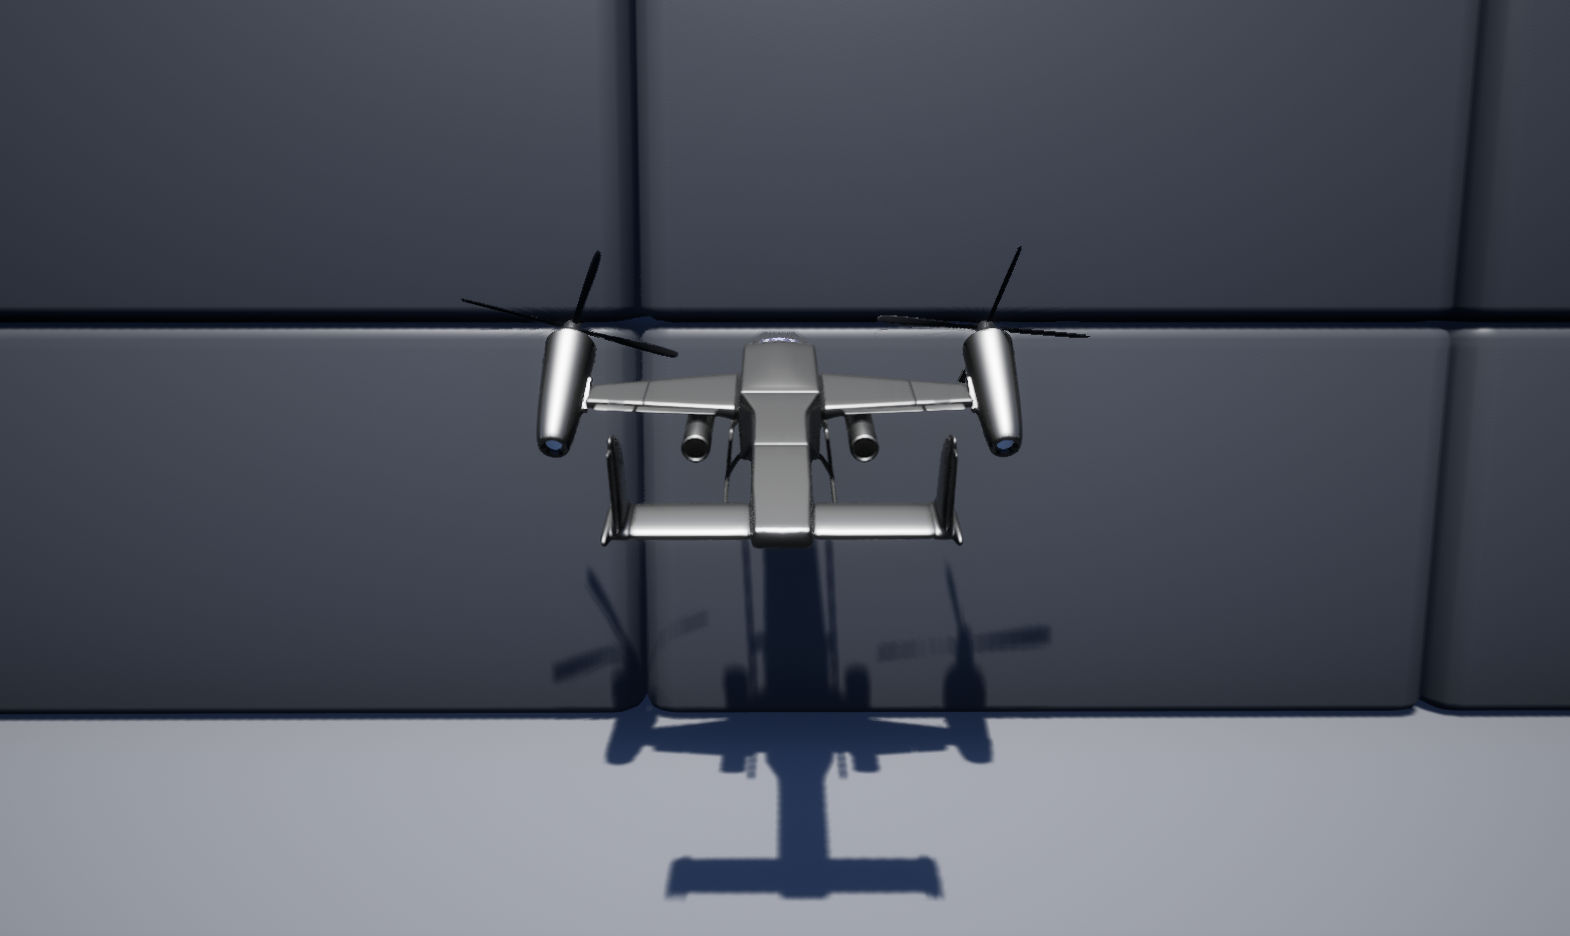
\includegraphics[width=\textwidth]{figures/homerpawn_final_flight}
    \caption[Custom aircraft flying in VTOL-AirSim]{
        The custom Homer aircraft flying in the Blocks world as it hits a wall.}%
    \label{fig:homerpawn_flight}
\end{figure}